% Copyright 2009--2014  Ed Bueler

\section{free boundary problems}

\begin{frame}{free boundary value problems}

\begin{itemize}
\item ice sheet/shelf modelling means free boundary problems
\item Hutter [1999] identifies some:
\end{itemize}
\begin{center}
  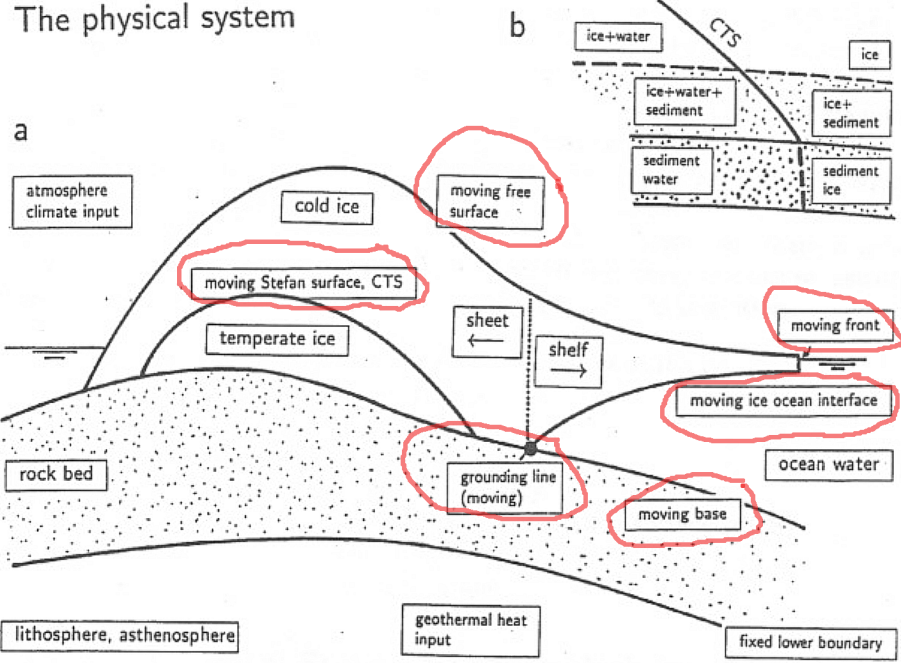
\includegraphics[width=0.8\textwidth]{freehutter}
\end{center}
\end{frame}


\begin{frame}{what is a ``free boundary''?}

\begin{itemize}
\item a \emph{free boundary} for a PDE is an unknown location at which there is a boundary condition
  \begin{itemize}
  \item[$\circ$] the location of the free boundary must be found at the same time as one solves the PDE problem
  \item[$\circ$] there must be enough additional information at a free boundary to determine its location
  \item[$\circ$] all free boundary problems are nonlinear, even if the PDE is linear
  \end{itemize}
\item classic \emph{example}:  consider an elastic membrane attached to a wire frame and stretched over an obstacle:
\end{itemize}

\begin{columns}
\begin{column}{0.5\textwidth}
\small
constraint:
  $$u \ge \psi$$

in locations where $u>\psi$, solve:
  $$\grad^2 u = 0$$
  
\emph{where is the free boundary, and what facts about $u$ are true there?}
\end{column}
\begin{column}{0.5\textwidth}
  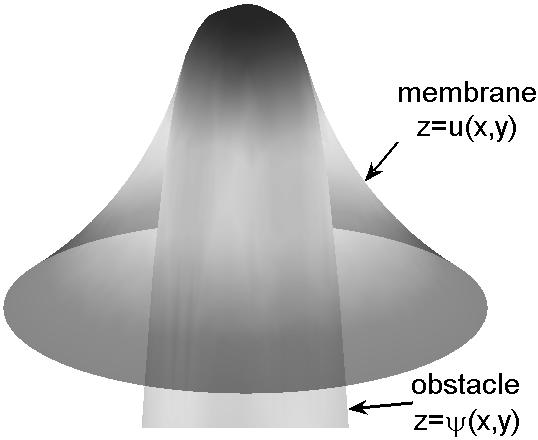
\includegraphics[width=1.0\textwidth]{classicalobs}
\end{column}
\end{columns}
\end{frame}


\begin{frame}{free boundary value problem 1: polythermal ice}

\small
\begin{itemize}
\item by volume, majority of ice sheet is \emph{cold} ($T < 0\phantom{|}^\circ\text{C}$)
\item \dots but there is some ice which is \emph{temperate}, where $T = 0\phantom{|}^\circ\text{C}$ \emph{and} there is a positive liquid fraction within the ice matrix
\item ice sheets are \emph{polythermal}
\item boundary between cold and temperate ice is ``CTS'' (= cold-temperate transition surface):
  \begin{itemize}
  \item[$\circ$] must be found, as free boundary, when solving conservation of energy equation (``Stefan problem'')
  \item[$\circ$] can be tracked explicitly [Greve, 1997]
  \item[$\circ$] or treated as a level surface of the enthalpy variable [Aschwanden et al, 2012]
  \end{itemize}
\end{itemize}

\begin{center}
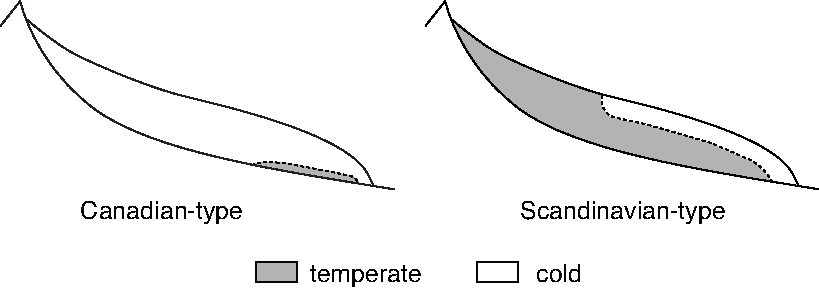
\includegraphics[width=0.8\textwidth]{polythermal_types}
\end{center}
\end{frame}


\begin{frame}{free boundary value problem 2: for ice streaming}

%\vspace{-0.2in}
\begin{itemize}
\item  Schoof's [2006] insight, for diagnostic case
  $$\text{SSA + (plastic till)} = \begin{pmatrix}
\text{well-posed free boundary problem} \\ \text{for location \emph{and} velocity of sliding}
\end{pmatrix} $$
\item ``plastic till'' means the basal strength (resistance) is given by a yield stress $\tau_c$:  \qquad $\vec\tau_b = \tau_c \mathbf{v}_b / |\mathbf{v}_b|$
\item Schoof's scheme is a \emph{whole ice sheet form} of MacAyeal's [1989] individual ice stream model
\end{itemize}

\begin{columns}
\begin{column}{0.5\textwidth}
\begin{center}
  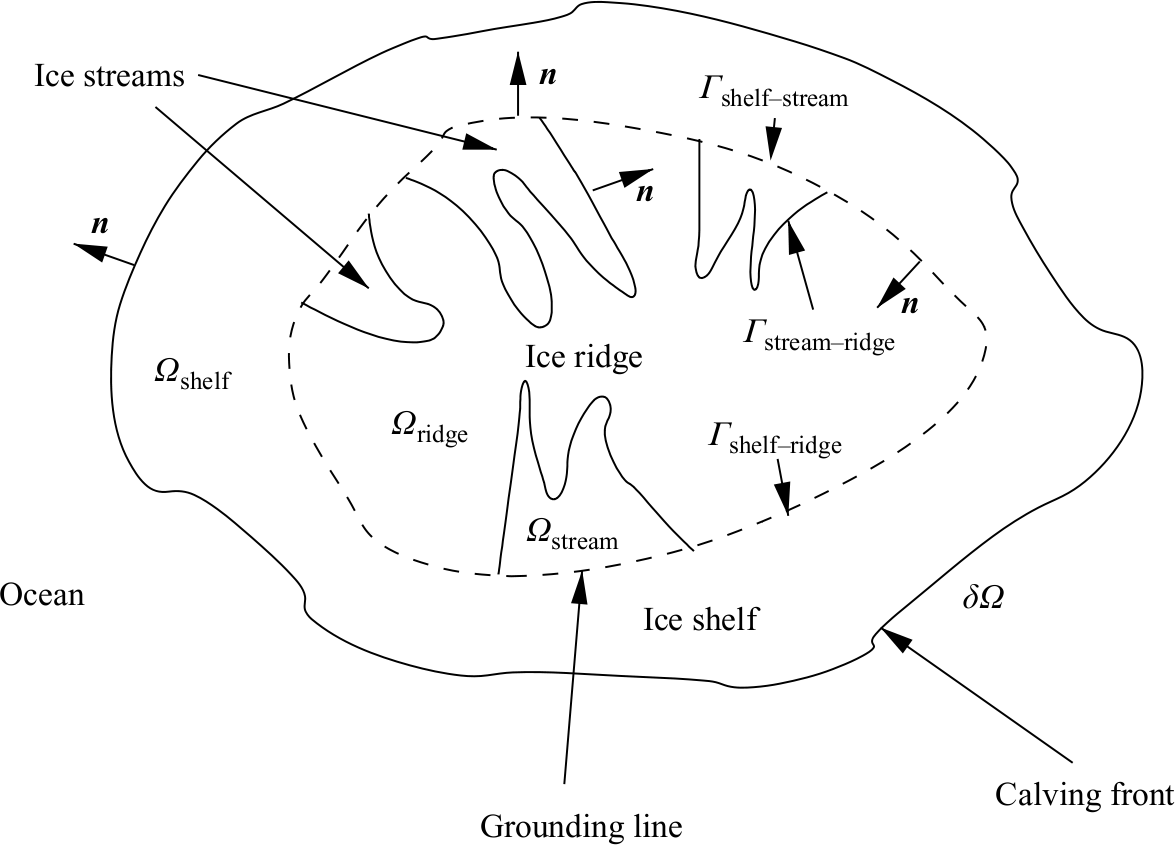
\includegraphics[width=1.0\textwidth]{schoof_planform}
\end{center}
\end{column}
\begin{column}{0.5\textwidth}
\begin{center}
  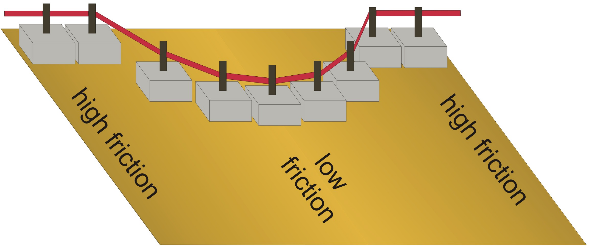
\includegraphics[width=0.95\textwidth]{schoof_sliders}
\end{center}
\end{column}
\end{columns}
\end{frame}


\begin{frame}{free boundary problem 3: for grounded ice sheet margin}

\begin{itemize}
\item side-by-side comparison, \emph{classical elastic membrane problem} versus \emph{steady ice sheet problem}
\item Jouvet \& Bueler [2012] show this is well-posed
\end{itemize}
\small
\begin{columns}[T]
\begin{column}{0.4\textwidth}
constraint:
  $$u \ge \psi$$

where $u>\psi$, solve:
  $$\grad^2 u = 0$$

\bigskip
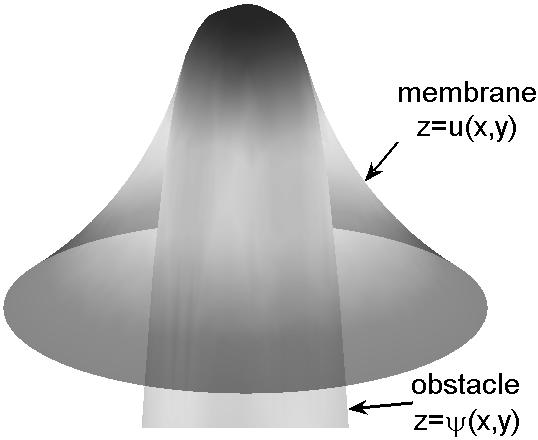
\includegraphics[width=0.8\textwidth]{classicalobs}
\end{column}
\begin{column}{0.6\textwidth}
constraint:
  $$h \ge b \qquad \iff \qquad H \ge 0$$

where $h>b$, solve steady SIA:
  $$0 = M + \Div \left(\Gamma H^{n+2} |\grad h|^{n-1} \grad h \right)$$

\bigskip
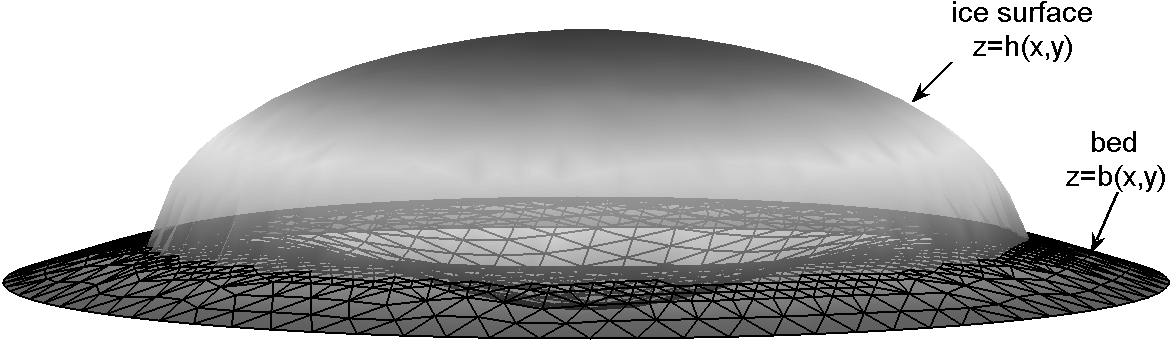
\includegraphics[width=0.9\textwidth]{capnonflatobs}
\end{column}
\end{columns}
\end{frame}


\begin{frame}{free boundary problems: why do they matter?}
\begin{itemize}
\item location of boundary may \emph{be} the glaciological question
\item free boundaries are always locations of \emph{loss of smoothness} relative to fixed boundary solutions
     \begin{itemize}
     \item[$\circ$] numerical errors dominated by errors near free boundaries 
     \item[$\circ$] are model results at free boundaries poor because of numerical problems or because of missing physical processes?
     \end{itemize}
\end{itemize}
\end{frame}